\documentclass{scrartcl}
\usepackage[utf8]{inputenc}
\usepackage{hyperref}
\usepackage{url}
\usepackage{natbib}
\usepackage{graphicx}
\usepackage{float}
\usepackage{listings}
\usepackage{xcolor}
\usepackage{booktabs}

\usepackage{cleveref} % this must be the last package to be loaded

\title{\LARGE
  Poool Game
}
\subtitle{Concurrent and Distributed Programming\\a.y. 2025--2026}

\author{
    Buda Marco \and Merighi Daniele \and Turchi Jacopo
}

\date{\today}

\begin{document}

\maketitle

\section{Problem Analysis}
\label{sec:problem_analysis}
This section provides a detailed analysis of the \texttt{Poool} game from a concurrent programming perspective. The main computational challenge resides in the simulation loop, which must continuously handle physics updates, boundary collisions, and elastic collisions among thousands of small balls (\texttt{MassiveBoardConf} configuration). 

The primary bottlenecks identified are:
\begin{itemize}
    \item \textbf{Linear State Updates:} Modifying positions and applying friction coefficients across large arrays of entities.
    \item \textbf{$O(n^2)$ Collision Resolution:} The nested loop required to evaluate and resolve simultaneous impacts between every pair of balls represents the highest density of CPU cycles.
\end{itemize}

\section{System Architecture and Architectural Design}
\label{sec:architecture}
The application is structured using the Model-View-Controller (MVC) pattern to separate core business data, synchronous rendering mechanics, and asynchronous command inputs. Two concurrent approaches have been implemented to scale processing requirements:

\subsection{Thread-Oriented Architecture (Platform Threads)}
This strategy divides the workload statically or cyclically among a set of long-running Java platform threads synchronized via custom \texttt{Latch} and \texttt{SynchBox} mechanisms.

\subsection{Task-Based Architecture (Executor Framework)}
This strategy decouples the synchronization layer by utilizing Java's \texttt{ExecutorService} pool. Tasks are submitted as fine-grained blocks of execution, allowing the underlying framework to handle optimal thread mapping and work distribution.

\subsection{Behavioral Modeling via Petri Nets}
% Placeholders for behavioral modeling descriptions and Petri net diagrams
\textit{[Insert Petri Net diagrams here to describe the lifecycle of the simulation loop, worker thread blocking states, and coordinator barrier synchronization.]}

\section{Performance Evaluation}
This section addresses the performance requirements of the assignment, specifically analyzing the advantage of the concurrent versions over the sequential one and evaluating the effectiveness of the program in exploiting available processing cores.

\subsection{Methodology}
Testing was conducted utilizing the \texttt{MassiveBoardConf} configuration (4500 entities) to generate a sufficiently compute-intensive workload. To ensure measurement accuracy, the physics and collision resolution logic (\texttt{updateState()}) was isolated. The Graphical User Interface was disabled to eliminate the interference of the sequential Swing Event Dispatch Thread.

Execution times were recorded using \texttt{System.nanoTime()}. Each configuration executed a 1000-update warm-up phase to allow the JVM Just-In-Time (JIT) compiler and Garbage Collector to stabilize, mitigating dynamic compilation overhead as described in "Performance of Concurrent Programs" slides. The following 2000 updates were measured, and the average execution time was calculated across 5 independent runs per configuration.

The baseline sequential execution time ($T_{seq}$) averaged 105.65ms per frame for the task version and 106.17ms for the thread one. The host system for the benchmark featured 12 available logical processors ($N_{cpu} = 12$).

\subsection{Concurrent vs. Sequential Advantage}
To evaluate how much the concurrent version improves upon the sequential one, Speedup ($S$) was calculated using the formula $S = T_{seq} / T_N$, where $T_N$ is the execution time with $N$ workers. 

\begin{table}[H]
    \centering
    \begin{tabular}{@{}lcccc@{}}
        \toprule
        \textbf{Workers ($N$)} & \textbf{Task Time (ms)} & \textbf{Thread Time (ms)} & \textbf{Task Speedup} & \textbf{Thread Speedup} \\ \midrule
        1 (Seq Baseline) & 105.65 & 106.17 & 1.00x & 1.00x \\
        2 & 55.96 & 56.76 & ,1.89x & 1.87x \\
        4 & 30.48 & 30.92 & 3.47x & 3.43x \\
        8 & 23.11 & 23.51 & 4.57x & 4.52x \\
        \textbf{12} & \textbf{16.74} & \textbf{18.31} & \textbf{6.31x} & \textbf{5.80x} \\
        13 & 21.92 & 22.67 & 4.82x & 4.68x \\ \bottomrule
    \end{tabular}
    \caption{Average execution time and Speedup for Task-Oriented and Thread-Oriented architectures.}
    \label{tab:speedup}
\end{table}

The empirical data demonstrates a definitive advantage of concurrent execution. The Task-Oriented implementation (utilizing the Executor framework) achieves a peak speedup of 6.31x at 12 workers, reducing the frame computation time from 105.65 ms to 16.74 ms. The Thread-Oriented architecture yields a similar peak speedup of 5.80x (18.31 ms). This confirms that distributing the physics workload across multiple active components substantially accelerates execution compared to the sequential variant.

\subsection{Core Exploitation and Scalability}
To assess how effectively the program exploits available cores, Efficiency ($E$) was calculated using the formula $E = S / N$. 

\begin{table}[H]
    \centering
    \begin{tabular}{@{}lcc@{}}
        \toprule
        \textbf{Workers ($N$)} & \textbf{Task Efficiency} & \textbf{Thread Efficiency} \\ \midrule
        1 & 1.00 & 1.00 \\
        2 & 0.94 & 0.94 \\
        4 & 0.86 & 0.86 \\
        8 & 0.57 & 0.56 \\
        \textbf{12} & \textbf{0.53} & \textbf{0.48} \\
        13 & 0.37 & 0.36 \\ \bottomrule
    \end{tabular}
    \caption{Computational Efficiency scaling per worker count.}
    \label{tab:efficiency}
\end{table}

\begin{figure}[H]
    \centering
    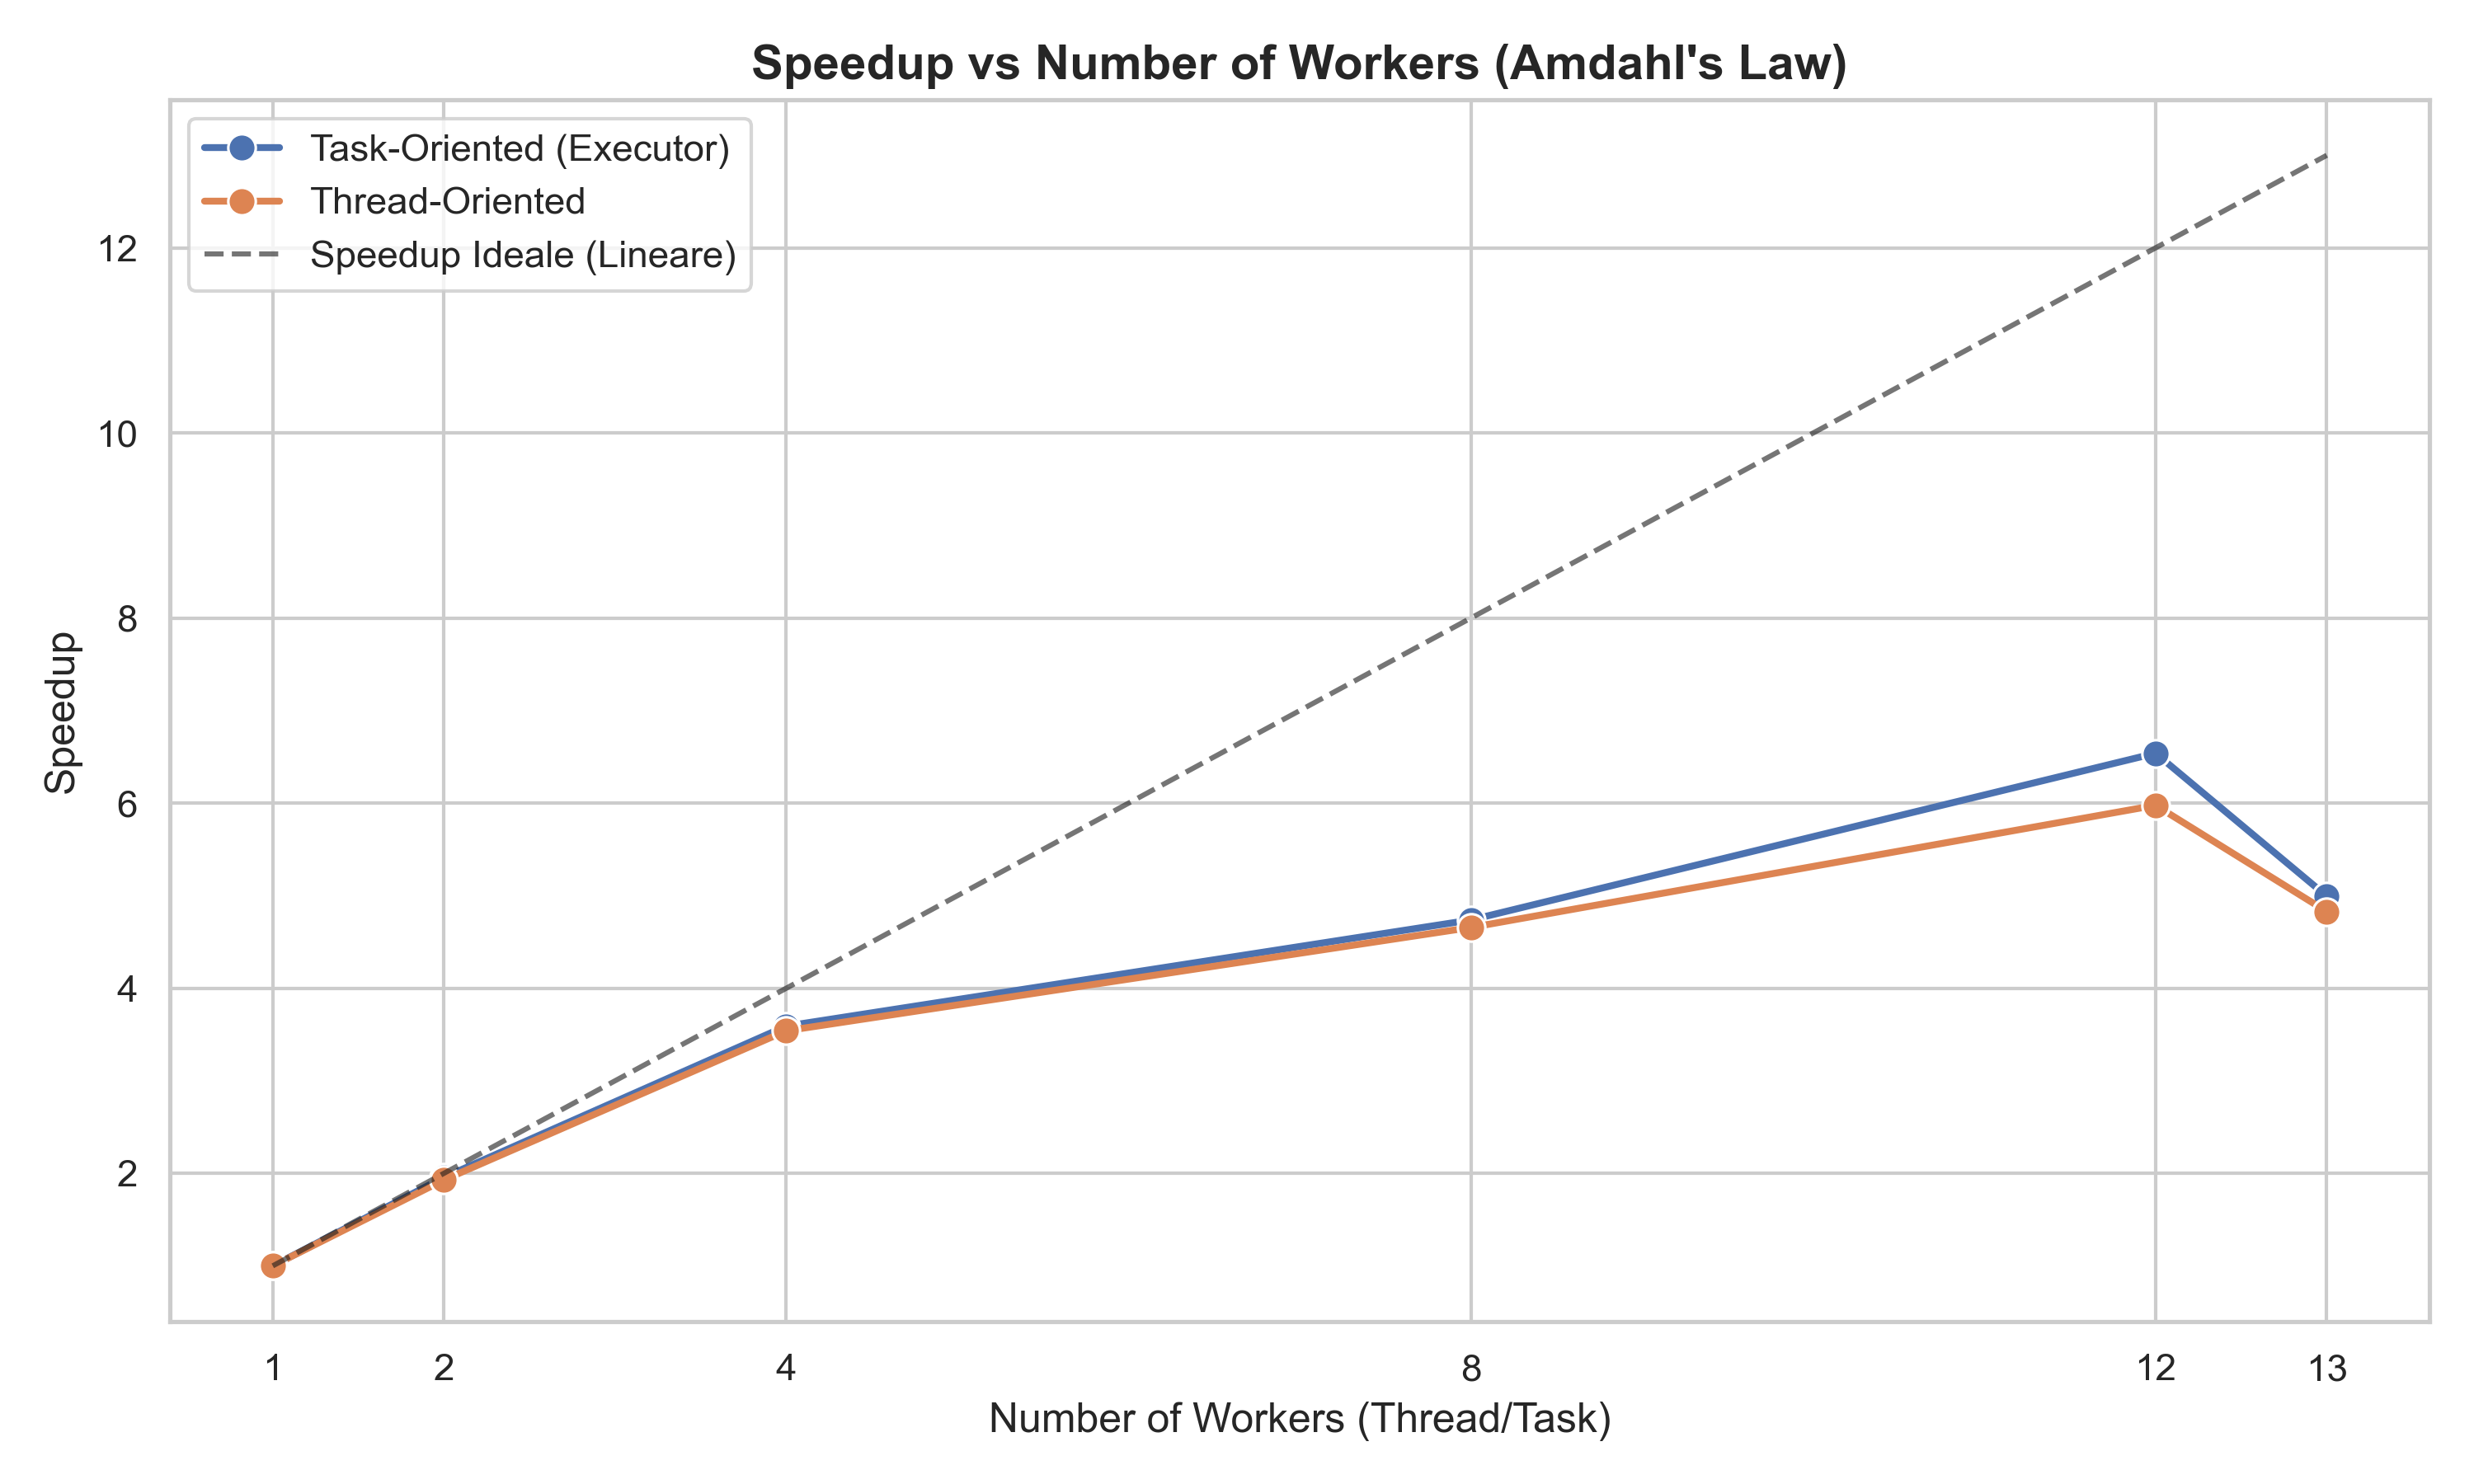
\includegraphics[width=0.9\textwidth]{images/speedup_plot.png} 
    \caption{Speedup scaling compared to the ideal linear trajectory.}
    \label{fig:speedup_plot}
\end{figure}

The application exhibits high efficiency ($> 89\%$) when scaling from 1 to 4 workers. The computation-heavy nature of the collision detection algorithm allows the processors to be exploited directly with minimal synchronization penalties. 

However, as dictated by Amdahl's Law, efficiency decays as the worker count increases. At 8 workers, efficiency drops to 59\%, and at the $N_{cpu}$ limit of 12 workers, it falls to 55\% (Task-Oriented). This sub-linear scaling is caused by multithreading costs, specifically context switching and lock contention over the shared structures tracking the game state. 

Testing with 13 workers ($N_{cpu} + 1$) caused a performance regression. While deploying $N_{cpu} + 1$ threads is a standard heuristic to prevent CPU cycle waste during page faults, the collision resolution task is strictly CPU-bound without blocking I/O operations. Consequently, oversubscribing the CPU forced thread scheduling overhead, dropping efficiency below 40\%. 

Overall, the Task-Oriented framework proved slightly more effective at exploiting cores than the Thread-Oriented approach, maintaining lower structural overhead per unit of work distributed.

\section{Program Verification and Model Checking}
\label{sec:verification}
This section covers the formal verification of safety and liveness properties using automated model-checking software.

\subsection{Java PathFinder (JPF) Configuration}
Formal verification was targets critical concurrency coordinates within the custom synchronization mechanisms, specifically focusing on validating \texttt{BoundedBufferImpl} and \texttt{LatchImpl} under high concurrency pressures.

\subsection{Verified Properties}
Using JPF, execution paths were explored to mathematically verify:
\begin{itemize}
    \item \textbf{Absence of Deadlocks:} Confirming that no interleaving of worker storage updates or coordinator latch requests results in a permanent stall state.
    \item \textbf{Race Condition Prevention:} Ensuring mutual exclusion during state modifications inside active monitor structures.
\end{itemize}


\end{document}